%%This is a very basic article template.
%%There is just one section and two subsections.
%\documentclass[12pt,oneside,a4paper,doublespacing]{article} % for submission
\documentclass[11pt,oneside]{article} % for sharing


\usepackage{appendix}
\usepackage{amsmath}
\usepackage{caption}
\usepackage{placeins}
\usepackage{graphicx}
\usepackage{subcaption}
\usepackage{longtable}
\usepackage{setspace}
%\usepackage{tikz}
\usepackage{booktabs}
\usepackage{xcolor,colortbl}
\usepackage{chngpage}
%\usepackage[active,tightpage]{preview}
\usepackage{natbib}
\bibpunct{(}{)}{,}{a}{}{;} 
\usepackage{url}
\usepackage{nth}
\usepackage{authblk}
%\usepackage{color}
%\usepackage{fontspec}
%\usepackage{pdfsync}

\renewcommand{\listtablename}{List of Appendix Tables}
\newcolumntype{C}[1]{>{\centering\let\newline\\\arraybackslash\hspace{0pt}}m{#1}}
\newcolumntype{L}[1]{>{\raggedright\let\newline\\\arraybackslash\hspace{0pt}}m{#1}}

% working on this need to concatenate file name based on sex and variable name
%\newcommand\Cell[1]{{\raisebox{-0.05in}{\includegraphics[height=.2in,width=.2in]{Figures/ColorCodes/\expandafter#1}}}}  

%%%%%%%%%%%%%%%%%%%%%%%%%%%%%%%%%%%%%%%%%%%%%%%%%%%%%%%%%%%%%%%%%%%%%%%%%%%%%
% setting color to letters affects spacing. Here's a hack I found here:
% http://tex.stackexchange.com/questions/212736/change-letter-colour-without-losing-letter-spacing
%\DeclareRobustCommand{\spacedallcaps}[1]{\MakeUppercase{\textsc{#1}}} % all
% caps with better spacing

%\colorlet{RED}{red}
%\colorlet{BLUE}{b}
\colorlet{rd}{red}
\colorlet{bl}{blue}

%%%%%%%%%%%%%%%%%%%%%%%%%%%%%%%%%%%%%%%%%%%%%%%%%%%%%%%%%%%%%%%%%%%%%%%%%%%%%%

\newcommand\ackn[1]{%
  \begingroup
  \renewcommand\thefootnote{}\footnote{#1}%
  \addtocounter{footnote}{-1}%
  \endgroup
}
\newcommand\vt[1]{\textcolor{rd}{#1}}
\newcommand\eg[1]{\textcolor{bl}{#1}}

\newcommand\tg[1]{\includegraphics[scale=.5]{Figures/triadtable/triad#1.pdf}}
\newcommand\tgh[1]{\raisebox{-.25\height}{\includegraphics[scale=.3]{Figures/triadtable/triad#1.pdf}}}

\defcitealias{HMD}{HMD}


\begin{document}

\title{A unified model of demographic time}

\author[1]{Tim Riffe\thanks{triffe@demog.berkeley.edu}}
\author[2]{Jonas Sch{\"o}ley}
\author[2]{Francisco Villavicencio}
\affil[1]{Max Planck Institute for Demographic Research}
\affil[2]{University of Southern Denmark}

%\author{[Authors]}

\maketitle

\begin{abstract}
We describe a three-dimensional model that relates six different aspects of
lifespans and time. The six aspects of demographic time considered are
chronological age, thanatological age, lifespan, year of birth, year of death,
and period. Two versions of the model are described: a relatively intuitive
extension of the right-angled Lexis diagram, and an isotropic extension based on
the regular tetrahedron. \ackn{The work reported in this manuscript was begun by
the first author while at the Department of Demography at the University of
California, Berkeley, and was supported by the U.S.
National Institute On Aging of the National Institutes of Health under award
numbers R01-AG011552 and R01-AG040245. The content is solely the responsibility of the authors and does not necessarily represent the official views of the funding agencies.}
\end{abstract}

The so-called Lexis diagram relates the chronological age (\eg{A}), period (\eg{P}),
and birth cohort (\eg{C}) indices of demographic time, \eg{APC}, but it does not account
for remaining years of life (thanatological age), and other related time
indices.
The thanatological counterpart to \eg{APC} is an identity between thanatological
age (\eg{T}), period (\eg{P}), and death cohort (\eg{D}), \eg{TPD}. A third
identity exists between chronological age (\eg{A}), thanatological age (\eg{T}), and lifespan (\eg{L}), \eg{ATL}, and a fourth between year of birth (\eg{C}), year of death (\eg{D}) and lifespan (\eg{L}), \eg{CDL}.
Each of these four triad identities may be sufficiently described by any
two of its consituent indices, making the third index redundant. Each of these
four identities also lacks a major dimension of time. The \eg{ATL} identity
lacks calendar time, the \eg{CDL} identity is ageless, \eg{APC} lacks an endpoint in time,
and \eg{TPD} lacks a starting point in time. We refer to these four identities
as triad identities.

To our knowledge, the only triad identity that has received serious
treatment at the time of this writing is the \eg{APC} identity. Different
aspects of the \eg{APC} identity have been discussed since at least 1868
\citep{knapp1868ermittlung}, and discussion remains lively today. Here it is our
objective to relate the six major indices of time in a geometric identity, in
much the same spirit as the work on \eg{APC} relationships done between the late
1860s and mid 1880s.\footnote{See e.g., \citet{keiding2011age} for an overview of that literature.} 

\subsection*{A tetrahedron relates the six time indices.}
Each of the four above-mentioned triad identities may be thought of as a
two-dimensional plane fully defined by any two of its three constituent time
indices.
In this case, we may imagine the third ``lacking'' dimension as providing
depth, for the sake of a mental image.
Having a non-redundant third dimension implies a multitude of parallel planes
for the given identity, each plane belonging to a unique value of the third time dimension. Any of the
identities can be extended in this way to fill a space. A space derived by
extending any of the triad identies into its lacking dimension implies each of the
other triad identities, making a total of six time indices. In essence, the
four triad identities may be thought of as parallel to the four faces of a
tetrahedron. In this case, the four ``lacking'' dimensions may be assigned to
the four vertices of the tetrahedron, and the six demographic time indices match
to the six edges of the tetrahedron. This three-dimensional construct
unifies the six indices of demographic time, and is the subject of this paper.

Let us first more rigorously define the previously-mentioned tetrahedron.
Luckily, the edges and vertices of a tetrahedron are easily rendered in a
two-dimensional graph, as seen in Figure~\ref{fig:tet}, with vertices labeled
in red and the six time indices labeled as blue edges.\footnote{The same graph
could be composed in four basic ways, depending on which vertex is in the
middle. These are given in an appendix.} The reader may also imagine this graph
as a transparent 3d object, in which case the four faces become aparent. There are two intuitive ways to imagine the graph as 3d, either the vertex \vt{4} is on top, and we gaze from a bird's-eye-view, or the
vertex \vt{4} is in the back, behind the other three vertices. Assume we
gaze from the top, for the sake of description. 

\begin{figure}[h!]
\centering
\caption{Graph of tetrahedron, with edges labeled by the six demographic time
indices.}
\label{fig:tet}
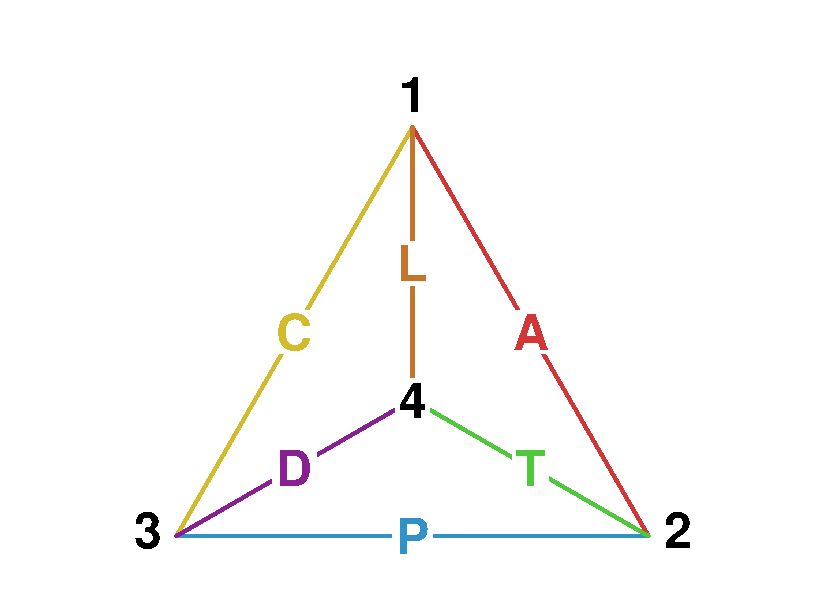
\includegraphics[scale=1]{Figures/TetraHedronVerticesEdges.pdf}
\end{figure}

\subsection*{Information criteria to derive the tetrahedron.}
The edges \eg{APC} at the base define the much-studied \eg{APC} plane. If the only
information we have is chronological age, period, and birth cohort (or just two
of these), then we have no access to the vertex \vt{4}. Each of the faces of the
tetrahedron has this quality. The South face \eg{TDP} has no access to \vt{1}.
The Northeast face, \eg{ATL} has no connection to \vt{3}, and the Northwest face
\eg{CDL} lacks a connection to \vt{2}. The triads that make up the faces of
the tetrahedron are stuck in ``flatland''. However, there are twenty ways in
total to choose three time indices from our total of six, and the four
above-named triads are the only four of these that will not yield the full 3d
space and imply the other three. The sixteen other combinations of three indices will recreate the full tetradhedron (hexad identity).

For example, say we are at vertex \vt{1}, and we therefore have
information on year of birth \eg{C}, completed lifespan \eg{L}, and
chronological age \eg{A}. Clearly, \eg{A} and \eg{C} imply \eg{P}
($\eg{C}+\eg{A}=\eg{P}$).
\eg{A} and \eg{L} imply \eg{T} ($\eg{L}-\eg{A}=\eg{T}$). Finally, \eg{C} and
\eg{L} imply \eg{D} ($\eg{C}+\eg{L}=\eg{D}$), and we have the full hexad
identity. In the tetrahedron graph, we have three edges that connect to the
four vertices. This is the essential property of a fully informed triad.

\begin{figure}[h!]
\centering
\caption{Graph of tetrahedron, edges eminating from vertice \vt{1} highlighted.}
\label{figtet4vert1}
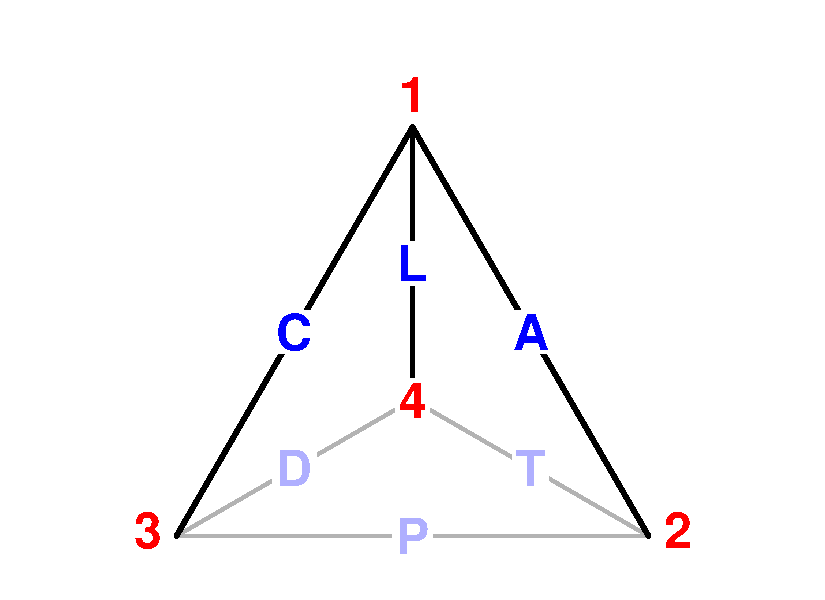
\includegraphics[scale=1]{Figures/tet4vert1.pdf}
\end{figure}
\noindent It is easily verified that each vertex has this property.
However, there are twelve other sets of three that also have this property. To locate
these ``hidden'' triads, first note that each index has an
opposite index, with which it shares no information. These pairs are
\eg{A-D}, \eg{L-P}, and \eg{C-T}, and can be found in Figure~\ref{fig:tet} as
the three sets of perpendicular edges. Each of these pairs can be completed into
a `fully-informed'' triad by the addition of any of the other four indices
(thereby connecting the edges). Doing so for each of the opposite pairs will
yield the remaining twelve triads.

\begin{table}[h]
\centering
\caption{All sets of three indices that imply the full six indices, graphed
given the previous orientation of the tetrahedron.}
\label{tab:set3}
\begin{tabular}{cccc}
\eg{ACD} & \eg{ACL} & \eg{ACT} & \eg{ADL}\\
\tg{ACD} & \tg{ACL} & \tg{ACT} & \tg{ADL}\\
\eg{ADP} & \eg{ADT} & \eg{ALP} & \eg{APT}\\
\tg{ADP} & \tg{ADT} & \tg{ALP} & \tg{APT}\\
\eg{CDP} & \eg{CDT} & \eg{CLP} & \eg{CLT}\\
\tg{CDP} & \tg{CDT} & \tg{CLP} & \tg{CLT}\\
\eg{CPT} & \eg{DLP} & \eg{DLT} & \eg{LPT}\\
\tg{CPT} & \tg{DLP} & \tg{DLT} & \tg{LPT}
\end{tabular}
\end{table}
\FloatBarrier
A like-organized table for the four triad identities simply highlights each of
the four faces of the tetrahedron, as seen in Table~\ref{tab:triadids}. When
graphed in this way, the vertex lacking a connection becomes clearer. We
therefore say that each of the triad identities is incomplete.

\begin{table}[h]
\centering
\caption{The four triad identities on the tetrahedron (same orientation)}
\label{tab:triadids}
\begin{tabular}{cccc}
\eg{APC} & \eg{TPD} & \eg{ATL} & \eg{CDL}\\
\tg{APC} & \tg{TPD} & \tg{ATL} & \tg{CDL}
\end{tabular}
\end{table}

Table~\ref{tab:set3} gives the full set of sixteen index-triads that are
complete in this sense. It can be verified that each of these
triads implies the full hexad identity. This property is comparable to the
reducibility characteristic of triad identities. For example, for the \eg{APC}
identity, the list of dyads that give full information is shorter:
\eg{AC}, \eg{AP}, \eg{PC}. The triads in Table~\ref{tab:set3} give analogous
information for the \eg{APCTDL} identity.
It may be further stated that no dyad of indices will give the hexad identity,
and any quad (or greater) of indices will yield the hexad identity. Any index
complemented by any index other than its opposite will imply one of
the triad identities.

\subsection*{The extension of time axes.}
We have said that planes defined by the four triad identities are parallel to
the faces of the the above-described tetrahedron. In imagining this three-dimensional
relationship, we are no longer confined to the extent of the tetrahedron that
we have used thus far for orientation. Instead each of its edges extends a
certain distance in either direction.
It may therefore help to first consider the extension of each axis (or index).
Some indices have a lower bound of zero and an upper bound set by the maximum
length of life, $\omega$, while others are boundless. \eg{A}, \eg{T}, and \eg{L}
are clearly in the range $[0,\omega]$.\footnote{It's best to imagine some number like 122.45 years, for $\omega$, rather than infinity. This is the longevity record at the time of this writing. Jeanne L. Calment would have had
$\eg{T}=122.45$ at birth, $\eg{A} = 122.45$ at death, and $\eg{L}=122.45$ for
her entire life.} \eg{P}, \eg{C}, and \eg{D} are bounded only by the inception and extinction of
our species, but may be thought of as boundless for practicality, or benchmarked
to our earliest and most recent observations for even more
practicality.\footnote{We explain the choice of the word ``benchmarked''. Say
we have a data series that runs from 1751 to 2011, and an upper age
interval of $110+$. Then we could say that \eg{P} is in the range $[1751,2011]$,
but by another reading, \eg{P} must range from at least as early as the earliest
\eg{C} and until at least as late as the latest \eg{D}. Someone dying at 110 in 1751
had a \eg{C} of 1640, and an infant born in 2011 that is destined to live to 110
will die in 2121. In this case a \eg{P} that \textit{contains} the observed
population will extend well before and after the observed data series, even
moreso if we take into account that $\omega > 110$.} As an abstraction,
however, the dimension of calendar time in this model is infinite. Of the four
triad identities, only one lacks an unbounded dimension, the \eg{ATL}. Adding
the absent dimension to \eg{ATL} therefore makes its 3d extension boundless. In
this way, we may imagine a prism-like construct, where \eg{A}, \eg{T}, and \eg{L}, compose
the faces of a triangular cross-section of said prism, which extends infinitely ``through'' the triangle.
We can think of the \eg{ATL} triangle passing through time, extending the population
forward to infinity. In this case, the \eg{ATL} triangle may take either the period
or cohort perspective, and this will be explained later. 

There are also
numerous ways that this three dimensional construct can be proportioned, of
which we present two in this paper. The first stems from the respect given to
right angles in the most common representation of the Lexis diagram. For this reason, it will likely be
the most intuitive rendition of the model, and it will be presented first. The
second version presented is isotropic with respect to time units in each of the
six temporal indices. In this case, the four tripartite identities are based on
equilateral triangles between their three constituent indices, and the four
planes are joined together such that each is parallel to a face from the regular
tetrahedron, a construct known in geometry as an octahedral-tetrahedral
honeycomb.

\section*{Intersecting planes}

The \eg{APC}, \eg{TPD}, \eg{ATL}, and \eg{CDL} planes can be conceived of as
\textit{compressions} of this 3d space, or as cross-sections of the 3d space. To
compress the space in this sense is to ignore the missing dimension,
whereas a cross-section sets a given triad identity against a particular
position of the missing dimension. \eg{APC} has typically been treated as a
compression, and myriad such examples are familiar to demographers.
A compressed \eg{TPD} diagram has thus far only appeared in \citet{pancho2015} as an aid in explaining a mathematical proof.
A cross-sectional \eg{ATL} diagram and surfaces have thus far only appeared in
\citet{riffe2015ttd}. This \eg{ATL} usage was selected for the 1915-1919 birth
cohort, and therefore belongs to the 3d space.

\subsection*{\eg{APC} \tgh{APC}}
The Lexis diagram has long been used in demography, both as a conceptual tool
for structuring data and observations, as inspiration for work on
statistical identification, and as the coordinate basis of contemporary
Lexis-surfaces.
Since the so-called Lexis diagram could have been named for others
\citep{vandeschrick2001lexis,keiding2011age}, and since we compare with other
temporal configurations, let us refer to it as the APC diagram, as seen in
Figure~\ref{APCright}
When a value (data) is structured by APC coordinates, we refer to it as an APC surface.

\begin{figure}[b!]
    \centering
    % figure made in R/LexisStandard.R
    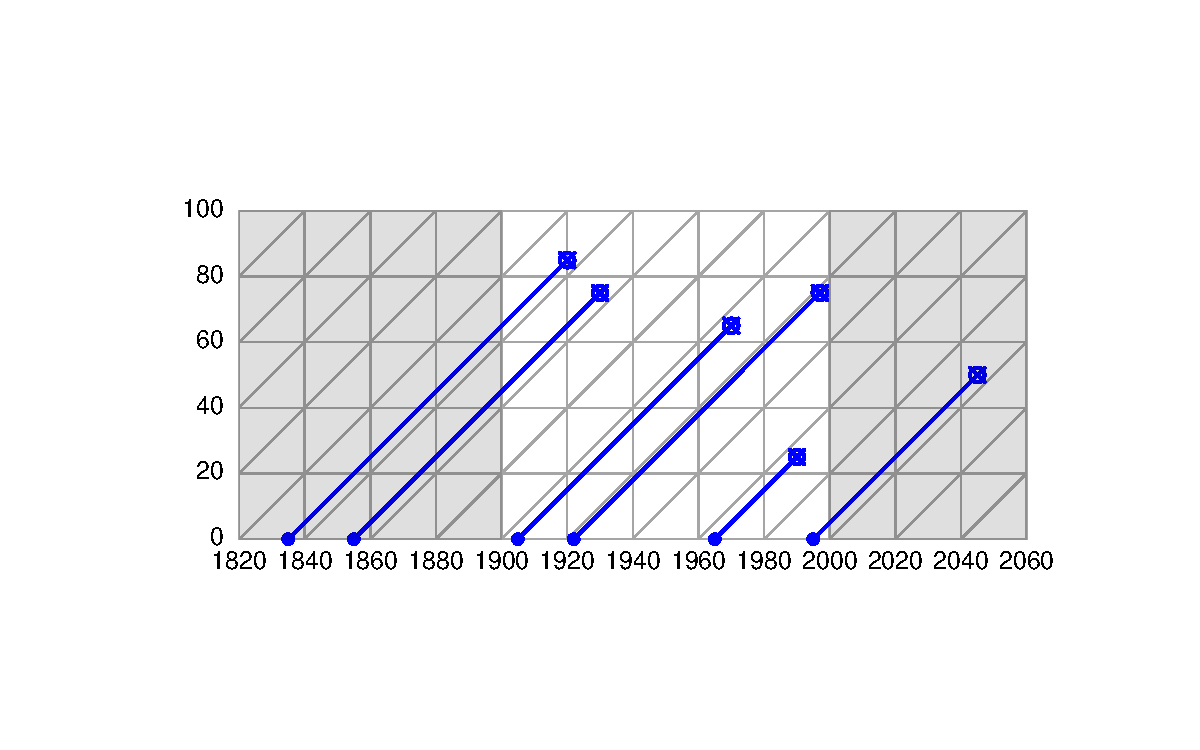
\includegraphics[scale=.7]{Figures/LabPres/APC4.pdf}
    \caption{Lifelines in the APC diagram}
    \label{APCright}
\end{figure} 

The APC diagram in Figure~\ref{APCright} represents years lived on the y axis,
calendar years on the x axis, and birth cohorts as the right-ascending
diagonals. This is the most common of several possible configurations
of the APC dimensions. Individual lifelines are aligned in the cohort direction,
starting with birth (filled circle) at chronological age zero, and death ()

Any APC surface can be interpreted along each of these
three dimensions of temporal structure. Such interpretation is a descriptive
task, and it does not succumb to problems of overidentification. Variation along
these three dimensions can not be parsimonsiously separated into the three
effects of A, P, and C. This is the so-called APC problem, and it is not the concern of the
present work. 

It has long been noted \citep{zeuner1869abhandlungen, perozzo1880della} that the
birth cohort dimension, as represented in Figure~\ref{APCright}, is relatively
longer than either the age or years axes. If a right angle and unity aspect
ratio is forced between any two of the APC dimensions, the third dimension is always be
stretched by $\sqrt{2}$. Another long-standing, but less common variant, is to
represent

\FloatBarrier

\subsection*{\eg{TPD} \tgh{TPD}}

Thanatological age (T), period (P) and death cohort (D) form a coordinate system
best imagined as the opposite of APC. One may take the same lifelines from
Figure~\ref{APCright} and realign them in descending fashion to create the
diagram in Figure~\ref{TPDright}

\begin{figure}[b!]
    \centering
    % figure made in R/LexisStandard.R
    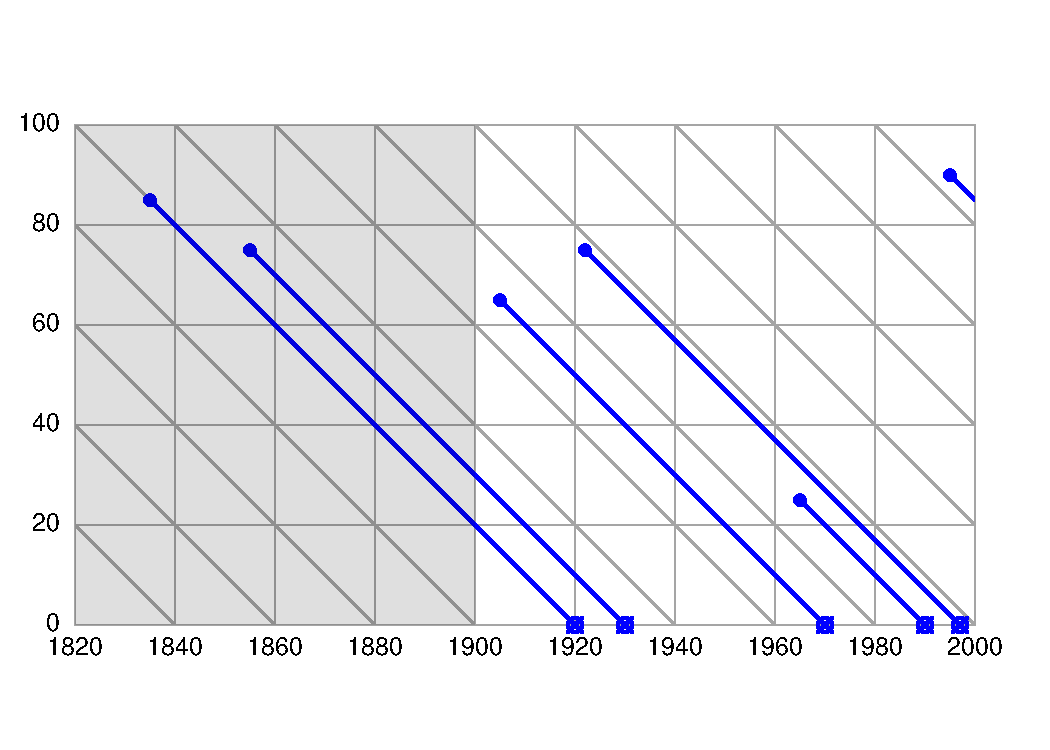
\includegraphics[scale=.7]{Figures/LabPres/TPD2.pdf}
    \caption{Lifelines in the TPD diagram}
    \label{TPDright}
\end{figure} 

\subsection*{\eg{ATL} \tgh{ATL}}
The second plane is ATL, a valid coordinate system for
processes that vary over the lifecourse, but not over time (P). Since the
lifecourse belongs to the cohort perspective, it is best to think of the ATL
plane as belonging to some particular birth cohort. Alternatively, an ATL
triangle may be taken as a cross-section along through the period dimension, a
sort of synthetic ATL plane.

\subsection*{\eg{CDL} \tgh{CDL}}

\section*{APCT}
I propose a geometric
identity that unifies all such temporal notions into a single (simple) spatial
relationship that serves as an omnibus conceptual aid to demographers, much as
the Lexis diagram does for APC relationships. The full result is a three
dimensional space that can be disected by any of four different planes,
each of which is parallel to the faces of a regular tetrahedron (see
Figure~\ref{fig:APCT} for a first mock-up of the model).
Each dissecting plane relates three indices of demographic time in proportion to one
another (1:1:1 ternary aspect ratio). The complete space can be described in
geometry nomenclature as the tetrahedral-octahedral honeycomb, which is a kind of space-filling tessellation.\footnote{Constructs following
this geometry exist both in nature and in man-made structures.} 
One of these planes is the familar Lexis plane (horizontal planes in
Figure~\ref{fig:APCT}, and the other three will be new surprises for
demographers. This three dimensional space is not only useful for the sake of formalizing observed temporal relationships, but also for encolosing
demographic time in the past and future (e.g., before the first census and after
the most recent census). 

\begin{figure}[!h]
\centering
\caption[cap]{A mock-up example of the unified model of demographic
time.\footnotemark}
\label{fig:APCT}
	\includegraphics[bb=0 0 3264 2448, width=\textwidth]{Figures/PhysicalModel.jpg}
\end{figure}
\footnotetext{This and other figures to be replaced with vector graphics, although
	I may bring this model to the presentation, since it helps explain concepts.}

A property of the geometry that I propose is that
the time units in every direction (with respect to each index) are proportional. The Lexis
diagram based on right angles and $45^\circ$ birth cohort lines does not have
this property, whereas Lexis diagrams and surfaces based on equilateral
triangles, such as some early proposals \citep[inter
alia, ][]{lexis1875einleitung, lewin1876rapport}, the masterful stereogram of
\citet{perozzo1880della}, or the more recent APC diagram
of \citet{ryder1980cohort}, do have this property. The disecting planes of the
model I propose are likewise composed of equilateral triangles. In Lexis
nomenclature, the 3d projections of an AP square, and AC or PC
parallelograms are all congruent shapes known as regular trigonal trapezohedra
(RTT). The orientation
of a given RTT uniquely defines the Lexis shape in question. Similar constructs
exist in the other time dimensions, and these will also be described. 
\FloatBarrier

\begin{appendices}
\section{Variants of tetrahedron graph}
The graph depicted in Figure~\ref{fig:tet} could be drawn with any of the
four vertices in the middle of the triangle (as well as other inversions
and rotations).
These would all serve equally well to present the same aspects of the model, and
we have no insight as to whether one of these renditions is more or less
intuitive. Figure~\ref{fig:app:tet} provides for perspectives on the
tetrahedron, for the case that this aids in understanding. The reader may make a
paper tetrahedron, with labeled edges and vertices to be convinced that
these are identical graphs.
\begin{figure*}
        \centering
        \caption{Some variants of the graph of the APCTDL tetrahedron.} 
         \label{fig:app:tet}
        \begin{subfigure}[b]{0.475\textwidth}
            \centering
            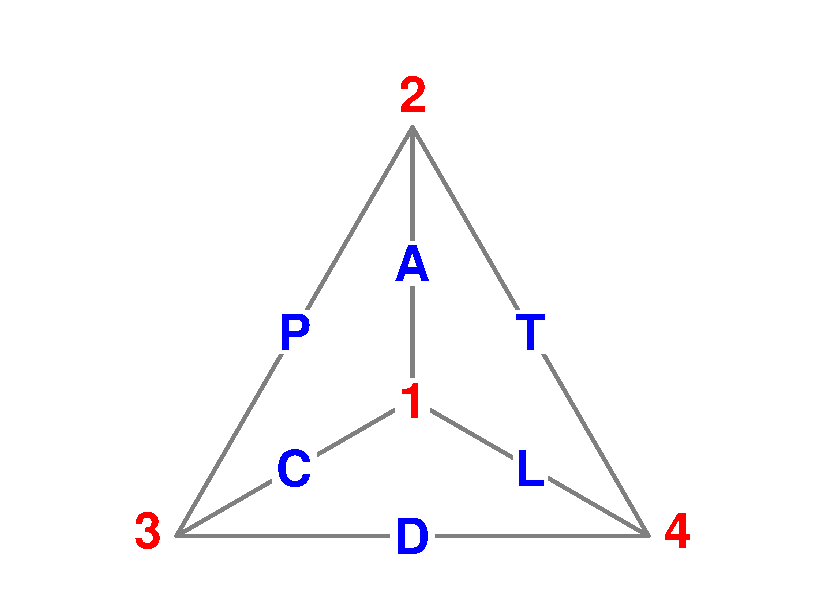
\includegraphics[width=\textwidth]{Figures/Tetra1.pdf}
           \caption{\small Vertex \vt{1} in middle. \eg{APC} Northwest.}
            \label{fig:tet1}
        \end{subfigure}
        \hfill
        \begin{subfigure}[b]{0.475\textwidth}  
            \centering 
            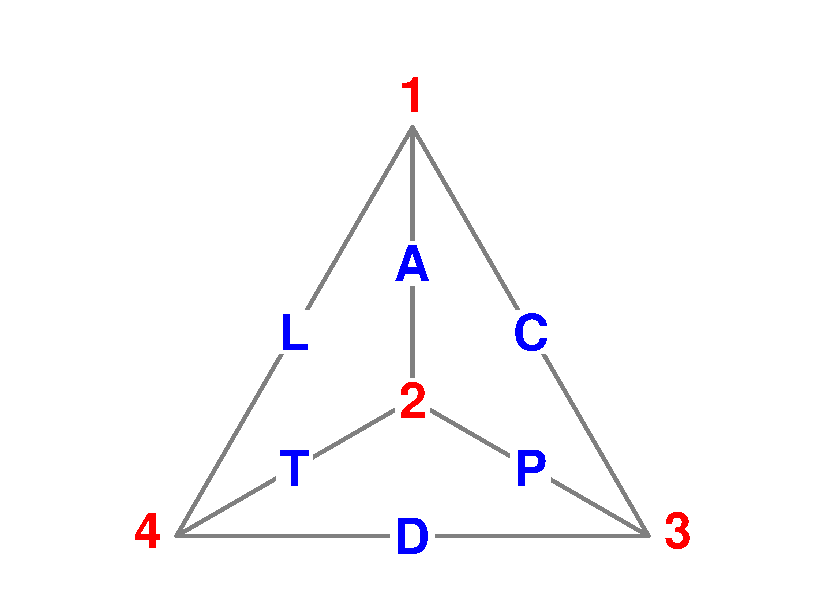
\includegraphics[width=\textwidth]{Figures/Tetra2.pdf}
           \caption{\small Vertex \vt{2} in middle. \eg{APC} Northeast.}
            \label{fig:tet2}
        \end{subfigure}
        \vskip\baselineskip
        \begin{subfigure}[b]{0.475\textwidth}   
            \centering 
            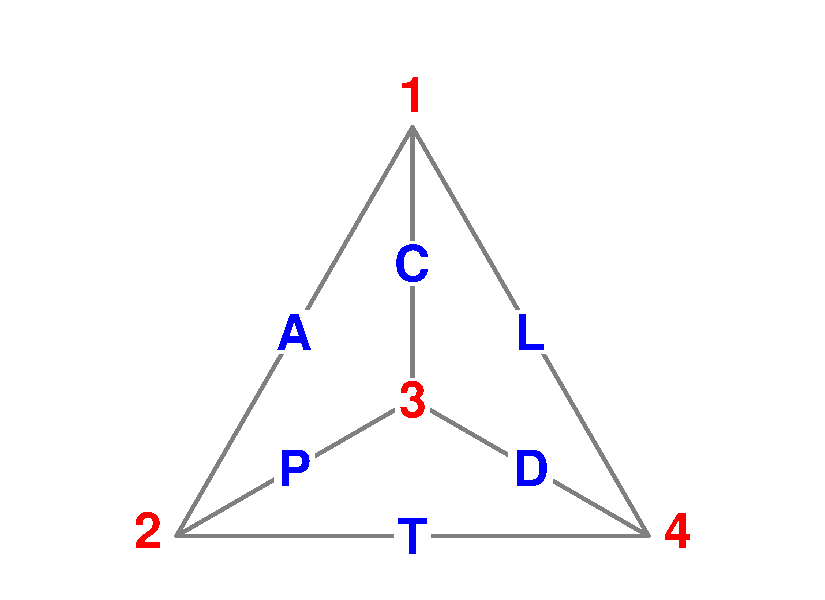
\includegraphics[width=\textwidth]{Figures/Tetra3.pdf}
           \caption{\small Vertex \vt{3} in middle. \eg{APC} Northwest.}
            \label{fig:tet3}
        \end{subfigure}
        \quad
        \begin{subfigure}[b]{0.475\textwidth}   
            \centering 
            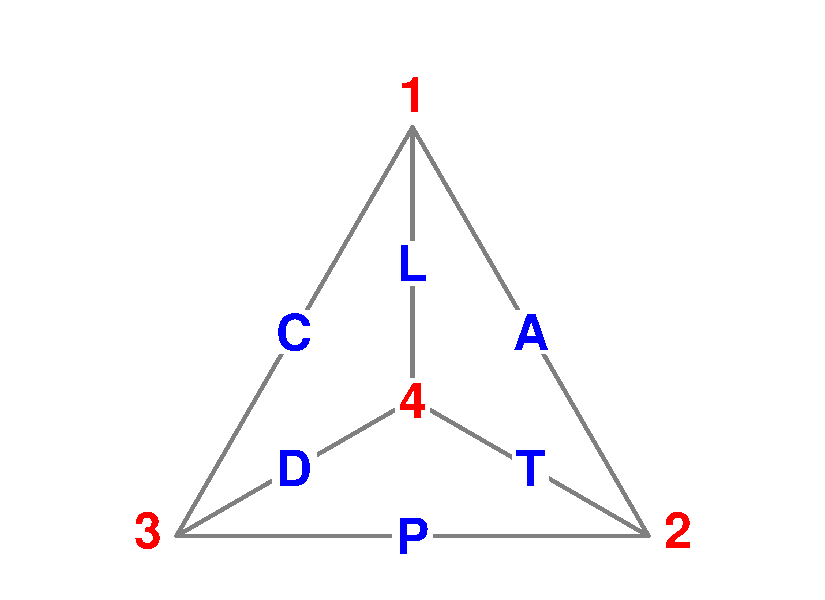
\includegraphics[width=\textwidth]{Figures/Tetra4.pdf}
            \caption{\small Vertex \vt{4} in middle, as in
            Figure~\ref{fig:tet}. \eg{APC} base.}
            \label{fig:tet4}
        \end{subfigure}
    \end{figure*}
\end{appendices}
\FloatBarrier

\bibliographystyle{plainnat}
  \bibliography{references} 



\end{document}